\documentclass[a4paper]{article}

\usepackage{inputenc}
\usepackage[british,UKenglish]{babel}
\usepackage{amsmath}
%\usepackage{titlesec}
\usepackage{color}
\usepackage{graphicx}
\usepackage{fancyref}
\usepackage{hyperref}
\usepackage{float}
\usepackage{scrextend}
\usepackage{setspace}
\usepackage{xargs}
\usepackage{multicol}
\usepackage{nameref}

\usepackage{sectsty}
\usepackage{multicol}
\usepackage{multirow}
\usepackage[procnames]{listings}
\usepackage{appendix}
\usepackage{geometry}
\usepackage{titlesec}

\newcommand\tab[1][1cm]{\hspace*{#1}}
\hypersetup{colorlinks=true, linkcolor=black}
\interfootnotelinepenalty=10000

\newcommand{\cleancode}[1]{\begin{addmargin}[3em]{3em}\texttt{\textcolor{cleanOrange}{#1}}\end{addmargin}}
\newcommand{\cleanstyle}[1]{\text{\textcolor{cleanOrange}{\texttt{#1}}}}


\usepackage[colorinlistoftodos,prependcaption,textsize=footnotesize]{todonotes}
\newcommandx{\commred}[2][1=]{\textcolor{Red}
{\todo[linecolor=red,backgroundcolor=red!25,bordercolor=red,#1]{#2}}}
\newcommandx{\commblue}[2][1=]{\textcolor{Blue}
{\todo[linecolor=blue,backgroundcolor=blue!25,bordercolor=blue,#1]{#2}}}
\newcommandx{\commgreen}[2][1=]{\textcolor{OliveGreen}{\todo[linecolor=OliveGreen,backgroundcolor=OliveGreen!25,bordercolor=OliveGreen,#1]{#2}}}
\newcommandx{\commpurp}[2][1=]{\textcolor{Plum}{\todo[linecolor=Plum,backgroundcolor=Plum!25,bordercolor=Plum,#1]{#2}}}

\def\code#1{{\tt #1}}

\def\note#1{\noindent{\bf [Note: #1]}}

\makeatletter
%% The "\@seccntformat" command is an auxiliary command
%% (see pp. 26f. of 'The LaTeX Companion,' 2nd. ed.)
\def\@seccntformat#1{\@ifundefined{#1@cntformat}%
   {\csname the#1\endcsname\quad}  % default
   {\csname #1@cntformat\endcsname}% enable individual control
}
\let\oldappendix\appendix %% save current definition of \appendix
\renewcommand\appendix{%
    \oldappendix
    \newcommand{\section@cntformat}{\appendixname~\thesection\quad}
}
\makeatother


% "define" Scala
\usepackage[T1]{fontenc}  
\usepackage[scaled=0.82]{beramono}  
\usepackage{microtype} 

\sbox0{\small\ttfamily A}
\edef\mybasewidth{\the\wd0 }

\lstdefinelanguage{scala}{
  morekeywords={abstract,case,catch,class,def,%
    do,else,extends,false,final,finally,%
    for,if,implicit,import,match,mixin,%
    new,null,object,override,package,%
    private,protected,requires,return,sealed,%
    super,this,throw,trait,true,try,%
    type,val,var,while,with,yield},
  sensitive=true,
  morecomment=[l]{//},
  morecomment=[n]{/*}{*/},
  morestring=[b]",
  morestring=[b]',
  morestring=[b]"""
}

\usepackage{color}
\definecolor{dkgreen}{rgb}{0,0.6,0}
\definecolor{gray}{rgb}{0.5,0.5,0.5}
\definecolor{mauve}{rgb}{0.58,0,0.82}

% Default settings for code listings
\lstset{frame=tb,
  language=scala,
  aboveskip=3mm,
  belowskip=3mm,
  showstringspaces=false,
  columns=fixed, % basewidth=\mybasewidth,
  basicstyle={\small\ttfamily},
  numbers=none,
  numberstyle=\footnotesize\color{gray},
  % identifierstyle=\color{red},
  keywordstyle=\color{blue},
  commentstyle=\color{dkgreen},
  stringstyle=\color{mauve},
  frame=single,
  breaklines=true,
  breakatwhitespace=true,
  procnamekeys={def, val, var, class, trait, object, extends},
  procnamestyle=\ttfamily\color{red},
  tabsize=2
}

\lstnewenvironment{scala}[1][]
{\lstset{language=scala,#1}}
{}
\lstnewenvironment{cpp}[1][]
{\lstset{language=C++,#1}}
{}
\lstnewenvironment{bash}[1][]
{\lstset{language=bash,#1}}
{}
\lstnewenvironment{verilog}[1][]
{\lstset{language=verilog,#1}}
{}



\lstset{frame=, basicstyle={\footnotesize\ttfamily}}
\geometry{left=3.17cm,right=3.17cm,top=2.54cm,bottom=2.54cm}
% 常规页眉页脚
\newpagestyle{main}{            
    \sethead{左页眉}{中页眉}{右页眉}     %设置页眉
    \setfoot{左页脚}{\thepage}{右页脚}      %设置页脚,可以在页脚添加 \thepage  显示页数
    \headrule                                      % 添加页眉的下划线
    \footrule                                       %添加页脚的下划线
}

% 封面页眉页脚
\newpagestyle{title}{            
    \sethead{报告号: 774323540--10dz1200500/01}{}{}     %设置页眉
%    \setfoot{左页脚}{\thepage}{右页脚}      %设置页脚,可以在页脚添加 \thepage  显示页数
    \headrule                                      % 添加页眉的下划线
    \footrule                                       %添加页脚的下划线
}

\pagestyle{main}

\graphicspath{ {images/} }
\usepackage{ctex}
\usepackage{caption}
\usepackage{subfigure}
%-----------------------------------------BEGIN DOC----------------------------------------

\begin{document}
\renewcommand{\contentsname}{目录}
\renewcommand{\appendixname}{附录}
\renewcommand{\appendixpagename}{附录}
\renewcommand{\refname}{参考文献} 
\renewcommand{\figurename}{图}
\renewcommand{\tablename}{表}
\renewcommand{\today}{\number\year 年 \number\month 月 \number\day 日}

\renewcommand{\maketitle}{
    \thispagestyle{title}
    \heiti
    \vspace*{94pt}
    \begin{center}
        \fontsize{50pt}{0} 科技报告\\
        \vspace*{300pt}
        \large \textcolor{red}{报告名称: \quad}\ \ \underline{\makebox[300pt]{陈家镇国际生态社区能源管理中心建设关键技术}}\\
        \large 支持渠道: \quad\ \ \underline{\makebox[300pt]{科技部等中央单位与上海市共同推进重大任务科研专项}}\\
        \large 报告类型: \quad\ \ \underline{\makebox[300pt]{最终报告}}\\
        \large 编制单位: \quad\ \ \underline{\makebox[300pt]{上海陈家镇建设发展有限公司}}\\
        \large 编制时间: \quad\ \ \underline{\makebox[300pt]{\today}}

    \end{center}
}

\maketitle

\newpage

%-----------------------------------------ABSTRACT-------------------------------------
\begin{center}
{\Large\bf{摘\ 要\\}}
\end{center}
请在这里输入摘要内容.
\newpage
%-----------------------------------------ABSTRACT-------------------------------------
\begin{center}
{\Large\bf{版\ 权\ 声\ 明\\}}
\end{center}
该文件受《中华人名共和国著作权法》的保护。ERCESI实验室保留拒绝授权违法复制该文件的权利。任何收存和保管本文件各种版本的单位和个人,未经ERCESI实验室(西北工业大学)同意,不得将本文档转借他人,亦不得随意复制、抄录、拍照或以任何方式传播。 否则,引起有碍著作权之问题,将可能承担法律责任。\newpage
%-----------------------------------------CONTENT-------------------------------------
\begin{center}
\tableofcontents\label{c}
\end{center}
\newpage

%------------------------------------------TEXT--------------------------------------------

%----------------------------------------OVERVIEW-----------------------------------------

%----------------------------------SYSTEM DESIGN------------------------------------------

\newpage
% -----------------------------------BLOCKS DESIGN----------------------------------------

%add more subsections for other block in you CPU design.

\section{基于Istio的协议实现}\label{baseistio}
传统的应用程序将所有功能都打包成一个独立的单元,因此也被称为单体应用。单体应用架构简单,在开发、测试和部署等方面都比较方便。但随着软件应用的发展,单体应用的弊端开始显现:不够灵活,对应用程序做任何细微的修改都需要将整个应用程序重新构建、重新部署,妨碍软件应用的持续交付;技术栈受限,开发团队的所有成员通常都必须使用相同的开发语言。因此,微服务架构应运而生。微服务架构将大型的单体应用拆分成若干个更小的服务,使得每个服务都可以独立地进行部署、升级、扩展和替换,服务间使用轻量级的通信协议进行通信(例如,同步的 REST,异步的 AMQP等),降低服务间耦合度的同时满足了软件程序对于快速持续集成和持续交付的需求。
\begin{figure}[ht]
 \centering
 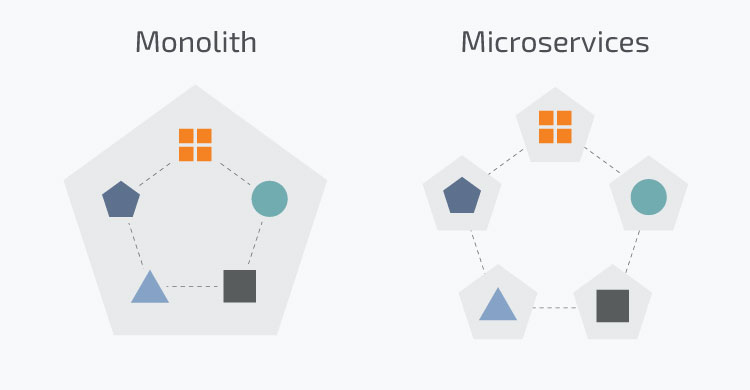
\includegraphics[height=5cm]{images/Microservices-vs-Monolith.jpg}
 \caption{单体应用和微服务应用}
 \label{fig:Microservices-vs-Monolith}
\end{figure}

与单体应用相比,微服务架构将系统应用的复杂度从单体应用内部的测试、部署、维护等转变到了微服务的连接调用、管理部署和监控等方面,因此微服务架构会极大地增加运维工作量,开发人员需要投入更多的精力来保证远程调用的可靠性与数据一致性。为了简化开发,开发人员通过典型的类库和框架(如Netflix OSS套件、Spring Cloud框架),编写较少的代码和注解就可以完成微服务间的服务发现、负载均衡、熔断、重试等功能。但此种办法缺点在于,开发人员需要掌握并熟练使用的内容较多,而且服务治理的功能不够齐全,很多功能需要自己进行拓展,编程语言也有所受限。这样所开发出来的微服务中,关键的业务逻辑代码和其它的用于管理服务间关系的非功能性代码混杂在一起。此时,若考虑为每一个微服务实例部署一个Sidecar,将所有前述的非功能性代码移到Sidecar中,由Sidecar来负责提供服务发现等辅助功能,而开发人员只需专注于微服务的业务逻辑,从而有效地进行了解耦。当为大型的微服务系统部署Sidecar时,微服务之间的服务调用关系便形成了服务网格(Service Mesh)。
\begin{figure}[ht]
 \centering
 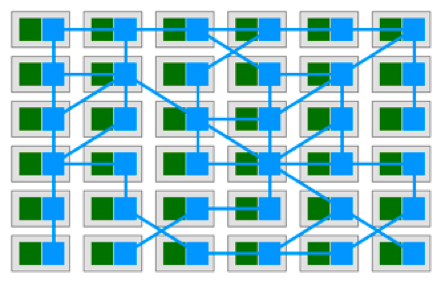
\includegraphics[]{images/service_mesh.png}
 \caption{服务网格(Service Mesh)}
 \label{fig:service_mesh}
\end{figure}

当前最主流的Service Mesh方案,是Google和IBM两个公司联合Lyft合作的开源项目Istio。在Istio的架构中,直接在Lyft开发的Envoy之上进行了拓展,然后将其作为Sidecar代理进行部署。Envoy Proxy作为数据面,除了提供服务发现、负载均衡、限流熔断等功能,还可以协调微服务的所有出入站流量,收集相关的性能指标,与控制面进行交互。而有了数据面的支持,控制面一方面通过Pilot组件下发配置信息到相应的Envoy Proxy中,负责流量管理,另一方面通过Mixer组件收集遥测数据,从而实现了对整个微服务系统多方面的掌管与监控。
\begin{figure}[ht]
 \centering
 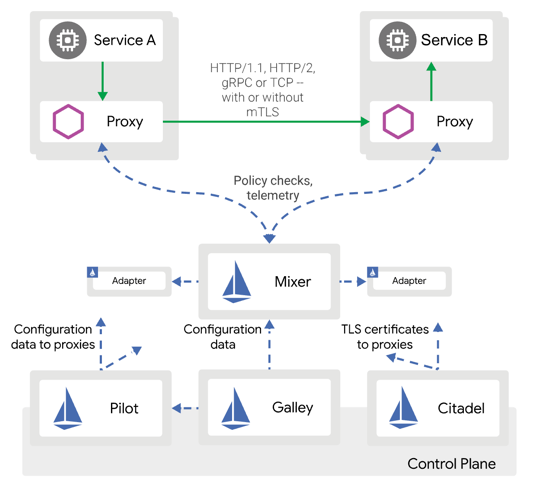
\includegraphics[height=7cm]{images/istio_arch.png}
 \caption{Istio架构图(v1.4)}
 \label{fig:istio_arch}
\end{figure}

基于Istio,部署前述的示例系统,具体架构变为\ref{fig:demo_arch_on_istio}。用户将访问请求发往Ingress Gateway,由Ingress Gateway依据相应的路由规则,再将请求转发至具体的后端服务中,然后收集运行结果并进行返回。每一次用户的请求都将产生一个分布式事务,其中可能会涉及多个服务的远程调用,但可以使用请求头中的x-b3-traceid字段进行唯一标识。Ingress Gaeway一方面将对应的服务接口暴露出来供用户进行访问,另一方面为用户屏蔽了后端服务的具体实现和路由转发等服务治理功能。

\begin{figure}[ht]
 \centering
 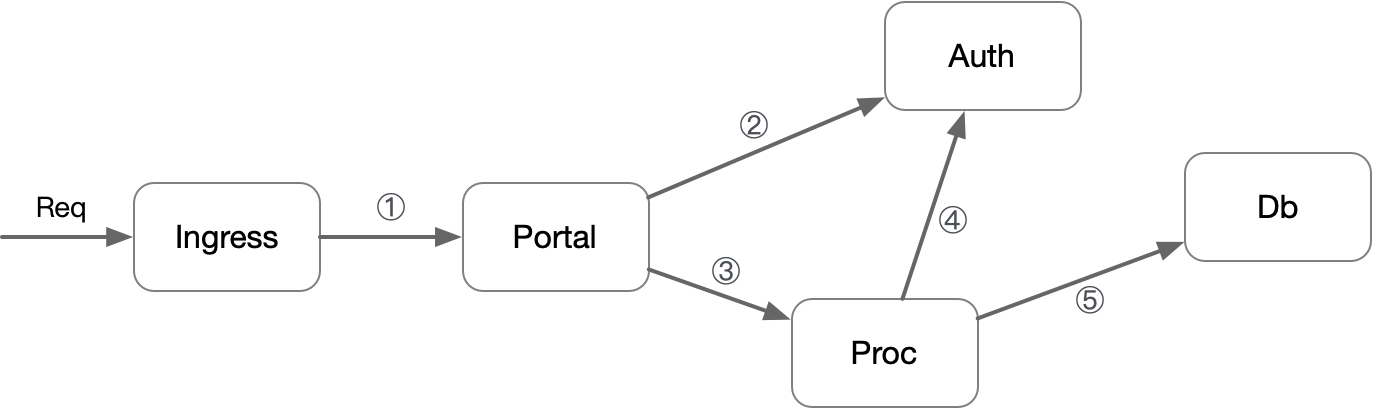
\includegraphics[height=4cm]{images/demo_arch_on_istio.png}
 \caption{Istio中的示例系统}
 \label{fig:demo_arch_on_istio}
\end{figure}

以示例系统中的auth-service服务为例,具体的实现和更新流程为:
\begin{enumerate}
	\item [0.] 插入Envoy容器和TraceManager容器:当每个服务实例部署时,我们将为每个服务实例对应部署Envoy容器和TraceManager容器。其中,Envoy容器负责从Istio控制面中接收用户的配置信息,然后将配置信息转换成对应的规则,对所有的出入站流量进行管理;与此同时,当存在具体的入站流量访问对应的服务时,Envoy会将此次分布式调用的唯一标识(x-b3-traceid)和相关信息发送至TraceManager中。而TraceManager容器则负责接收从Envoy容器中发送过来的信息,对其进行记录管理,为后续的更新过程提供支持。插入的Envoy和TraceManager容器分别作为客户端和服务端,通过Unix Domain Socket的方式进行通信,从而最大程度地减少了消息传送对Envoy快速处理用户请求的影响。
	\begin{figure}[ht]
	 \centering
	 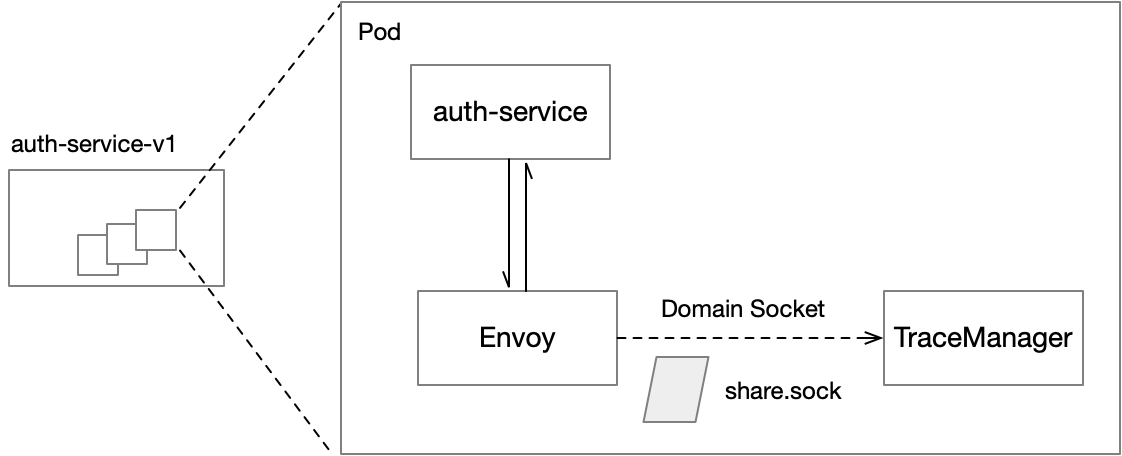
\includegraphics[height=5cm]{images/insert_containers.png}
	 \caption{插入容器}
	 \label{fig:insert_containers}
	\end{figure}

	\item [1.] 创建初始的路由规则和版本信息:当整个系统部署完成时,为每个服务创建初始的路由规则和版本信息。图\ref{fig:vs_all_v1}中定义了路由规则,要求流量调用到auth-service时,所有流量都发往v1版本,且在返回的头信息中会带上自定义的信息,后续将利用此头信息进行流量的转发;图\ref{fig:dr_v1}中定义了版本信息,说明带有{version: v1}标签的所有auth-service的服务实例都属于v1版本;此时系统的运行状态对应显示为图\ref{fig:traffic_all_v1}
	\begin{figure}[htbp]
	\centering
	\begin{minipage}[t]{0.48\textwidth}
	\centering
	\centerline{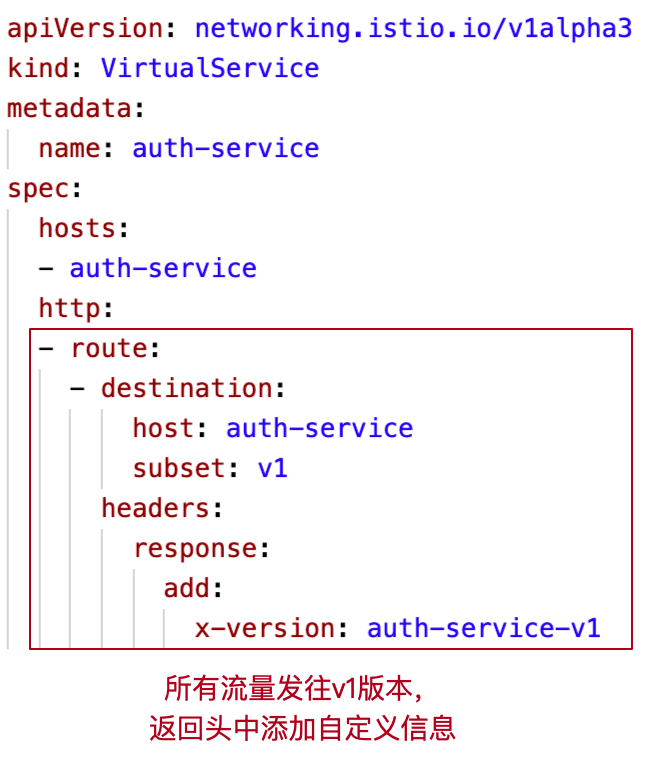
\includegraphics[width=6cm]{vs_all_v1.png}}
	\caption{v1路由规则}
	\label{fig:vs_all_v1}
	\end{minipage}
	\begin{minipage}[t]{0.48\textwidth}
	\centering
	\centerline{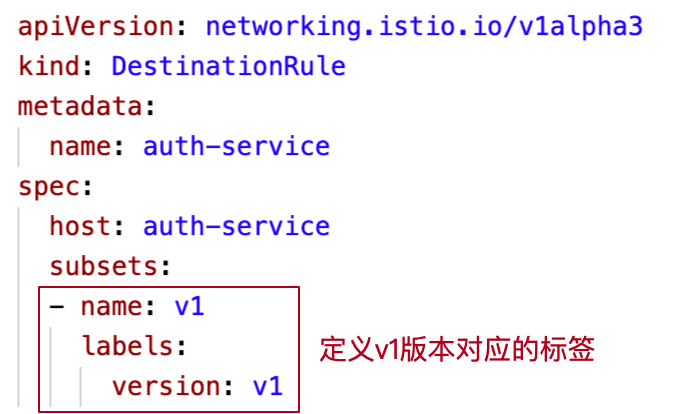
\includegraphics[width=6cm]{dr_v1.png}}
	\caption{v1版本规则}
	\label{fig:dr_v1}
	\end{minipage}
	\end{figure}

	\begin{figure}[ht]
	 \centering
	 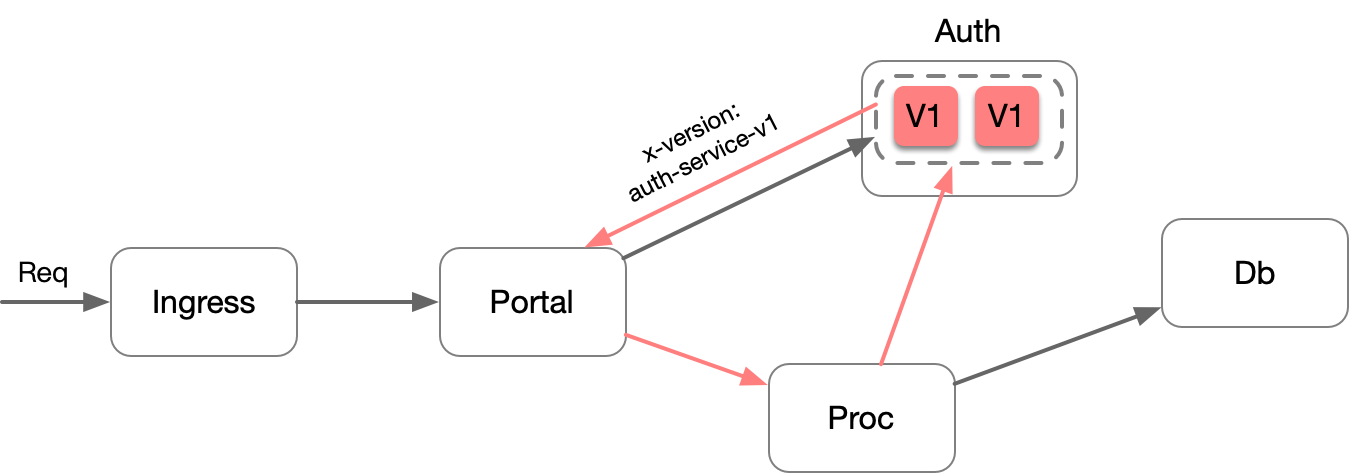
\includegraphics[height=4cm]{images/traffic_all_v1.png}
	 \caption{流量全部发往v1}
	 \label{fig:traffic_all_v1}
	\end{figure}

	在系统的运行过程中,当存在入站流量调用到auth-service时,Envoy容器执行拦截操作:一方面将流量转发往负责的服务实例,另一方面将此次调用所对应的traceid信息从头信息中提取出来并发送往TraceManager容器,TraceManager容器则将对应的traceid存到对应的TraceidSet中,该集合代表了当前所有调用过auth-service的用户请求;同时,当本次用户请求处理完成并返回Ingress Gateway时,Ingress Gateway实例内部会执行同样的添加操作,这里的TraceidSet则代表了当前已完成并返回的用户请求集合。
	\begin{figure}[ht]
	 \centering
	 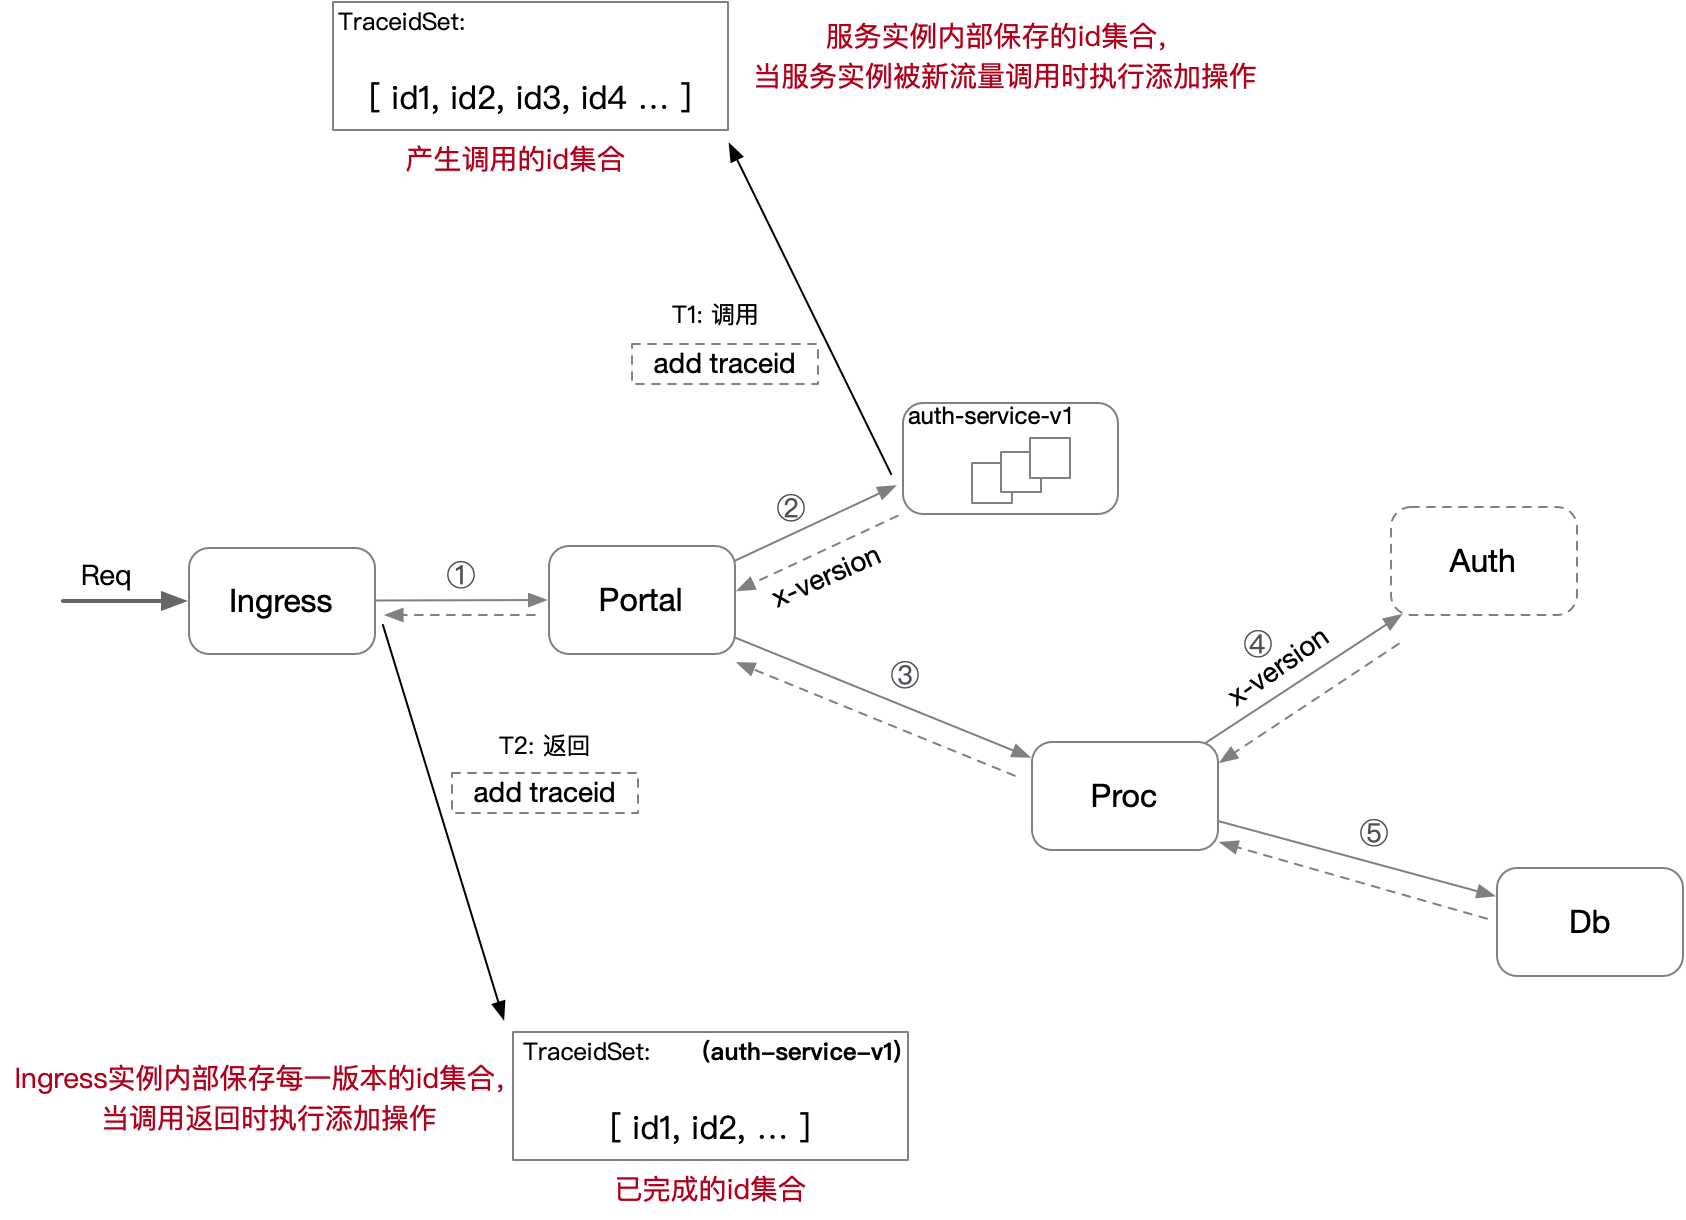
\includegraphics[height=10cm]{images/record_trace.png}
	 \caption{事务记录}
	 \label{fig:record_trace}
	\end{figure}

	\item [2.] 新版本上线

	\item [3.] 配置更新
	\item [4.] 旧版本撤销请求
	\item [5.] 
\end{enumerate}

\newpage
\section{人机物融合平台架构与技术集成} 

互联网的快速发展催生新技术与新业务的出现。软件从单纯的信息处理环节逐步成为了应用价值观的主要载体,并形成将人、计算机以及物理世界相连接的人机物融合软件新形态。人机物融合平台旨在人机物三元融合开放多变的环境下,灵活地协同管理各种自治的资源,支撑人机物融合应用系统的运行。

\subsection{总体的设计和结构}

人机物融合平台的运行环境基于当前最主流的容器化编排系统Kubernetes,在其上制定了一套人机物资源的描述规范,设计了一种消息驱动的人机物资源协作模型,构建了一套面向人机物融合的资源服务治理框架。

\subsection{人机物资源的描述与编排}
  实际的物理资源都要抽象成一种数据结构存储在系统中,系统同时要更新和维护它们。本软件平台通过Kubernetes CRD在系统中表示抽象资源,存储在etcd中,Kubernetes Controller负责维护它们,同步状态。
\subsubsection{人机物资源描述规范}
CRD是CustomResourceDefinition的简写,资源是kubernetes中的抽象概念,CRD是自定义的资源。

所有物理资源都要在系统中注册,且在系统中表达为Resource CRD,需要使用一些参数描述资源。这些参数告诉了Kubernetes平台如何去访问资源并维护资源的状态。首先,资源需要一个唯一的标识。其次,因为需要使用探针去采集资源的各项信息,需要包含探针程序的镜像地址和启动命令以及启动参数。
\subsubsection{人机物资源的运行时编排(WHG)}
Resource CRD由Resource Controller管理,控制器监控资源的状态,当监测资源的增删改事件时就会生成一个包含相关资源名称的request塞入工作队列,Reconcile方法每隔很短的一段时间被调用一次,从工作队列中取出一个request作为参数进行处理。

Reconcile首先根据request中包裹的资源名称和命名空间找到Resource的实例,如果是删除事件什么都不需要做,增改事件则会根据ProbeEnabled字段判断是否需要新建、更新、删除探针Deployment资源。
\subsection{消息驱动的人机物资源协作模型}
\subsubsection{资源状态的同步}
\subsubsection{资源代理服务(TC)}
\subsubsection{消息队列(TC)}

\subsection{面向人机物融合的资源服务治理框架}
\subsubsection{人机物融合场景下的服务路由(TC)}
\subsubsection{资源服务的动态更新(WDY)}
% -----------------------------------Appendix----------------------------------------
% -----------------------------------REFERENCE----------------------------------------
\end{document}

